\documentclass{standalone}
\usepackage{tikz}
\usetikzlibrary{patterns, positioning}


\begin{document}
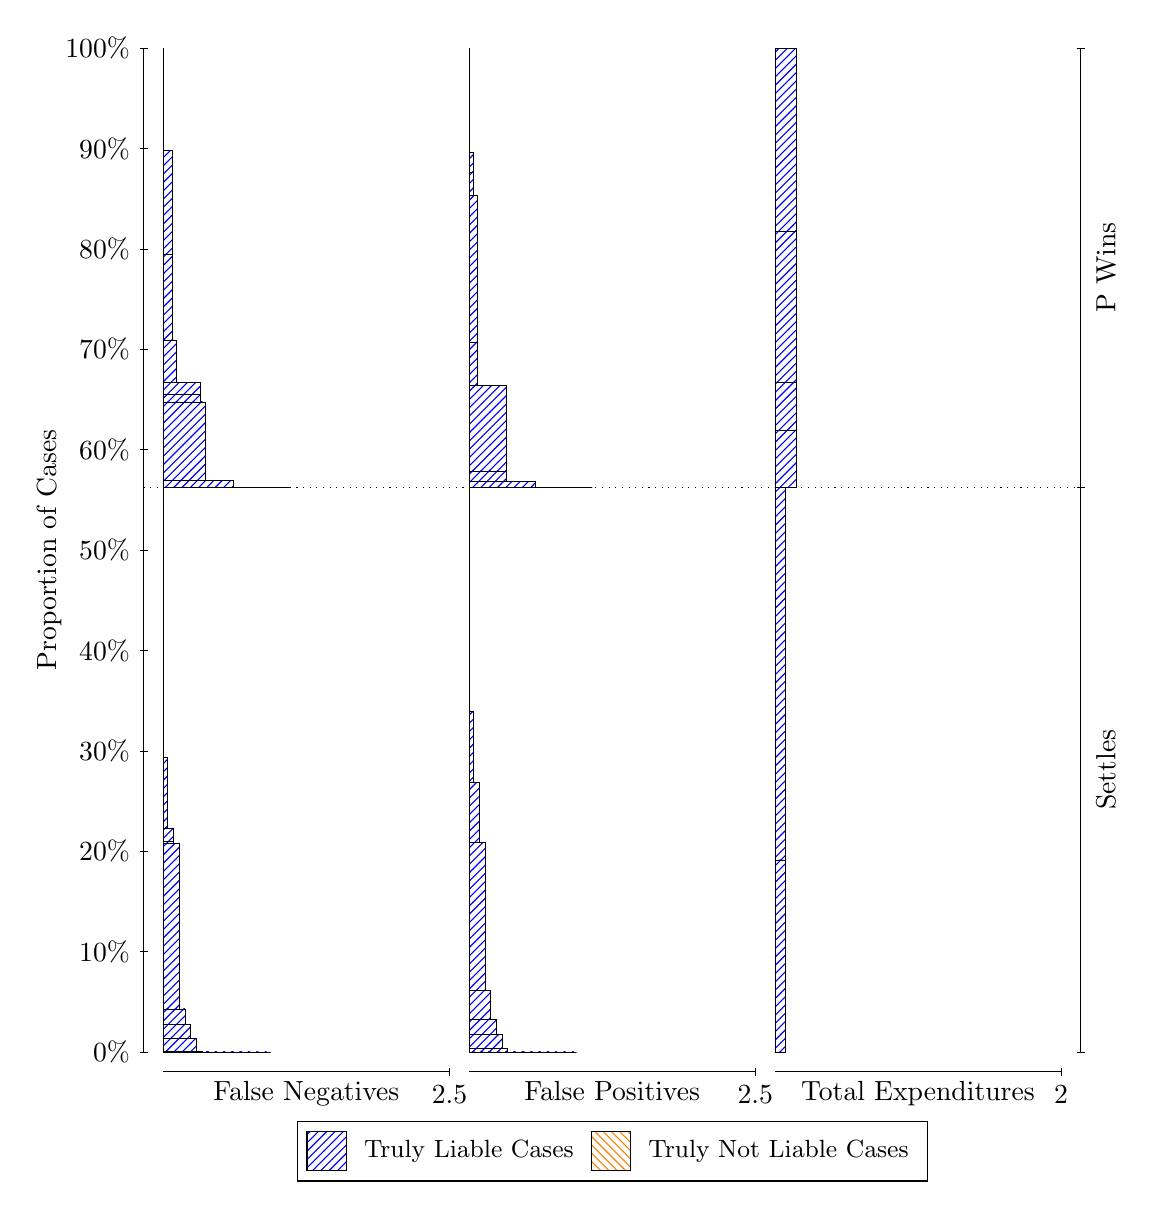
\begin{tikzpicture}
\draw[black, very thin] (1.5,1.75) -- (1.5,14.5);
\node[rotate=90, text=black, anchor=center] at (0.3, 8.125) {Proportion of Cases};
\draw[black, very thin] (1.45,1.75) -- (1.55,1.75);
\node[text=black, anchor=east] at (1.45, 1.75) {0\%};
\draw[black, very thin] (1.45,3.025) -- (1.55,3.025);
\node[text=black, anchor=east] at (1.45, 3.025) {10\%};
\draw[black, very thin] (1.45,4.3) -- (1.55,4.3);
\node[text=black, anchor=east] at (1.45, 4.3) {20\%};
\draw[black, very thin] (1.45,5.575) -- (1.55,5.575);
\node[text=black, anchor=east] at (1.45, 5.575) {30\%};
\draw[black, very thin] (1.45,6.85) -- (1.55,6.85);
\node[text=black, anchor=east] at (1.45, 6.85) {40\%};
\draw[black, very thin] (1.45,8.125) -- (1.55,8.125);
\node[text=black, anchor=east] at (1.45, 8.125) {50\%};
\draw[black, very thin] (1.45,9.4) -- (1.55,9.4);
\node[text=black, anchor=east] at (1.45, 9.4) {60\%};
\draw[black, very thin] (1.45,10.675) -- (1.55,10.675);
\node[text=black, anchor=east] at (1.45, 10.675) {70\%};
\draw[black, very thin] (1.45,11.95) -- (1.55,11.95);
\node[text=black, anchor=east] at (1.45, 11.95) {80\%};
\draw[black, very thin] (1.45,13.225) -- (1.55,13.225);
\node[text=black, anchor=east] at (1.45, 13.225) {90\%};
\draw[black, very thin] (1.45,14.5) -- (1.55,14.5);
\node[text=black, anchor=east] at (1.45, 14.5) {100\%};

\draw[black, very thin] (13.4,1.75) -- (13.4,14.5);
\draw[black, very thin] (13.35,1.75) -- (13.45,1.75);
\node[anchor=west] at (13.35, 1.75) {};
\draw[black, very thin] (13.35,8.9204) -- (13.45,8.9204);
\node[anchor=west] at (13.35, 8.9204) {};
\draw[black, very thin] (13.35,14.5) -- (13.45,14.5);
\node[anchor=west] at (13.35, 14.5) {};

\draw[black, very thin, pattern color=blue, pattern=north east lines] (1.75,1.75) rectangle (3.1125,1.75);
\draw[black, very thin, pattern color=blue, pattern=north east lines] (1.75,1.75) rectangle (2.9672,1.75);
\draw[black, very thin, pattern color=blue, pattern=north east lines] (1.75,1.75) rectangle (2.8218,1.75);
\draw[black, very thin, pattern color=blue, pattern=north east lines] (1.75,1.75) rectangle (2.7492,1.75);
\draw[black, very thin, pattern color=blue, pattern=north east lines] (1.75,1.75) rectangle (2.6765,1.75);
\draw[black, very thin, pattern color=blue, pattern=north east lines] (1.75,1.75) rectangle (2.6038,1.75);
\draw[black, very thin, pattern color=blue, pattern=north east lines] (1.75,1.75) rectangle (2.5312,1.7504);
\draw[black, very thin, pattern color=blue, pattern=north east lines] (1.75,1.7504) rectangle (2.4585,1.7507);
\draw[black, very thin, pattern color=blue, pattern=north east lines] (1.75,1.7507) rectangle (2.3858,1.7509);
\draw[black, very thin, pattern color=blue, pattern=north east lines] (1.75,1.7509) rectangle (2.3132,1.7521);
\draw[black, very thin, pattern color=blue, pattern=north east lines] (1.75,1.7521) rectangle (2.2405,1.7552);
\draw[black, very thin, pattern color=blue, pattern=north east lines] (1.75,1.7552) rectangle (2.1678,1.9256);
\draw[black, very thin, pattern color=blue, pattern=north east lines] (1.75,1.9256) rectangle (2.0952,2.0958);
\draw[black, very thin, pattern color=blue, pattern=north east lines] (1.75,2.0958) rectangle (2.0225,2.2966);
\draw[black, very thin, pattern color=blue, pattern=north east lines] (1.75,2.2966) rectangle (1.9498,4.3956);
\draw[black, very thin, pattern color=blue, pattern=north east lines] (1.75,4.3956) rectangle (1.8772,4.4275);
\draw[black, very thin, pattern color=blue, pattern=north east lines] (1.75,4.4275) rectangle (1.8772,4.5964);
\draw[black, very thin, pattern color=blue, pattern=north east lines] (1.75,4.5964) rectangle (1.8045,5.4961);
\draw[black, very thin, pattern color=orange, pattern=north west lines] (1.75,5.4961) rectangle (1.75,5.4961);
\draw[black, very thin, pattern color=blue, pattern=north east lines] (1.75,5.4961) rectangle (1.75,8.9204);
\draw[black, very thin, pattern color=blue, pattern=north east lines] (1.75,8.9204) rectangle (3.3668,8.9204);
\draw[black, very thin, pattern color=blue, pattern=north east lines] (1.75,8.9204) rectangle (3.0035,8.9215);
\draw[black, very thin, pattern color=blue, pattern=north east lines] (1.75,8.9215) rectangle (2.949,8.9215);
\draw[black, very thin, pattern color=blue, pattern=north east lines] (1.75,8.9215) rectangle (2.6402,9.0132);
\draw[black, very thin, pattern color=blue, pattern=north east lines] (1.75,9.0132) rectangle (2.5857,9.0133);
\draw[black, very thin, pattern color=blue, pattern=north east lines] (1.75,9.0133) rectangle (2.2768,10.007);
\draw[black, very thin, pattern color=blue, pattern=north east lines] (1.75,10.007) rectangle (2.2223,10.102);
\draw[black, very thin, pattern color=blue, pattern=north east lines] (1.75,10.102) rectangle (2.2223,10.25);
\draw[black, very thin, pattern color=blue, pattern=north east lines] (1.75,10.25) rectangle (1.9135,10.793);
\draw[black, very thin, pattern color=blue, pattern=north east lines] (1.75,10.793) rectangle (1.859,11.883);
\draw[black, very thin, pattern color=blue, pattern=north east lines] (1.75,11.883) rectangle (1.859,13.203);
\draw[black, very thin, pattern color=orange, pattern=north west lines] (1.75,13.203) rectangle (1.75,13.203);
\draw[black, very thin, pattern color=blue, pattern=north east lines] (1.75,13.203) rectangle (1.75,14.5);
\draw[black, very thin, pattern color=orange, pattern=north west lines] (5.6333,1.75) rectangle (6.9958,1.75);
\draw[black, very thin, pattern color=blue, pattern=north east lines] (5.6333,1.75) rectangle (6.9958,1.75);
\draw[black, very thin, pattern color=orange, pattern=north west lines] (5.6333,1.75) rectangle (6.7052,1.75);
\draw[black, very thin, pattern color=blue, pattern=north east lines] (5.6333,1.75) rectangle (6.7052,1.75);
\draw[black, very thin, pattern color=blue, pattern=north east lines] (5.6333,1.75) rectangle (6.6325,1.75);
\draw[black, very thin, pattern color=orange, pattern=north west lines] (5.6333,1.75) rectangle (6.5598,1.75);
\draw[black, very thin, pattern color=blue, pattern=north east lines] (5.6333,1.75) rectangle (6.5598,1.75);
\draw[black, very thin, pattern color=orange, pattern=north west lines] (5.6333,1.75) rectangle (6.4145,1.75);
\draw[black, very thin, pattern color=blue, pattern=north east lines] (5.6333,1.75) rectangle (6.4145,1.7504);
\draw[black, very thin, pattern color=blue, pattern=north east lines] (5.6333,1.7504) rectangle (6.3418,1.7504);
\draw[black, very thin, pattern color=orange, pattern=north west lines] (5.6333,1.7504) rectangle (6.2692,1.7504);
\draw[black, very thin, pattern color=blue, pattern=north east lines] (5.6333,1.7504) rectangle (6.2692,1.7521);
\draw[black, very thin, pattern color=blue, pattern=north east lines] (5.6333,1.7521) rectangle (6.1965,1.7521);
\draw[black, very thin, pattern color=orange, pattern=north west lines] (5.6333,1.7521) rectangle (6.1238,1.7521);
\draw[black, very thin, pattern color=blue, pattern=north east lines] (5.6333,1.7521) rectangle (6.1238,1.7987);
\draw[black, very thin, pattern color=blue, pattern=north east lines] (5.6333,1.7987) rectangle (6.0512,1.9691);
\draw[black, very thin, pattern color=orange, pattern=north west lines] (5.6333,1.9691) rectangle (5.9785,1.9691);
\draw[black, very thin, pattern color=blue, pattern=north east lines] (5.6333,1.9691) rectangle (5.9785,2.1642);
\draw[black, very thin, pattern color=blue, pattern=north east lines] (5.6333,2.1642) rectangle (5.9785,2.1656);
\draw[black, very thin, pattern color=blue, pattern=north east lines] (5.6333,2.1656) rectangle (5.9058,2.5363);
\draw[black, very thin, pattern color=orange, pattern=north west lines] (5.6333,2.5363) rectangle (5.8332,2.5363);
\draw[black, very thin, pattern color=blue, pattern=north east lines] (5.6333,2.5363) rectangle (5.8332,4.4087);
\draw[black, very thin, pattern color=blue, pattern=north east lines] (5.6333,4.4087) rectangle (5.8332,4.409);
\draw[black, very thin, pattern color=blue, pattern=north east lines] (5.6333,4.409) rectangle (5.7605,5.1743);
\draw[black, very thin, pattern color=blue, pattern=north east lines] (5.6333,5.1743) rectangle (5.6878,6.074);
\draw[black, very thin, pattern color=blue, pattern=north east lines] (5.6333,6.074) rectangle (5.6333,8.9204);
\draw[black, very thin, pattern color=orange, pattern=north west lines] (5.6333,8.9204) rectangle (7.1957,8.9204);
\draw[black, very thin, pattern color=blue, pattern=north east lines] (5.6333,8.9204) rectangle (7.1957,8.9204);
\draw[black, very thin, pattern color=orange, pattern=north west lines] (5.6333,8.9204) rectangle (6.8323,8.9204);
\draw[black, very thin, pattern color=blue, pattern=north east lines] (5.6333,8.9204) rectangle (6.8323,8.9212);
\draw[black, very thin, pattern color=orange, pattern=north west lines] (5.6333,8.9212) rectangle (6.469,8.9212);
\draw[black, very thin, pattern color=blue, pattern=north east lines] (5.6333,8.9212) rectangle (6.469,8.9948);
\draw[black, very thin, pattern color=orange, pattern=north west lines] (5.6333,8.9948) rectangle (6.4145,8.9948);
\draw[black, very thin, pattern color=blue, pattern=north east lines] (5.6333,8.9948) rectangle (6.4145,8.9948);
\draw[black, very thin, pattern color=orange, pattern=north west lines] (5.6333,8.9948) rectangle (6.1057,8.9948);
\draw[black, very thin, pattern color=blue, pattern=north east lines] (5.6333,8.9948) rectangle (6.1057,9.1286);
\draw[black, very thin, pattern color=blue, pattern=north east lines] (5.6333,9.1286) rectangle (6.1057,10.217);
\draw[black, very thin, pattern color=orange, pattern=north west lines] (5.6333,10.217) rectangle (6.0512,10.217);
\draw[black, very thin, pattern color=blue, pattern=north east lines] (5.6333,10.217) rectangle (6.0512,10.218);
\draw[black, very thin, pattern color=blue, pattern=north east lines] (5.6333,10.218) rectangle (5.7423,10.761);
\draw[black, very thin, pattern color=blue, pattern=north east lines] (5.6333,10.761) rectangle (5.7423,12.628);
\draw[black, very thin, pattern color=orange, pattern=north west lines] (5.6333,12.628) rectangle (5.6878,12.628);
\draw[black, very thin, pattern color=blue, pattern=north east lines] (5.6333,12.628) rectangle (5.6878,12.916);
\draw[black, very thin, pattern color=blue, pattern=north east lines] (5.6333,12.916) rectangle (5.6878,13.171);
\draw[black, very thin, pattern color=blue, pattern=north east lines] (5.6333,13.171) rectangle (5.6333,14.5);
\draw[black, very thin, pattern color=orange, pattern=north west lines] (9.5167,1.75) rectangle (9.6529,1.75);
\draw[black, very thin, pattern color=blue, pattern=north east lines] (9.5167,1.75) rectangle (9.6529,4.1887);
\draw[black, very thin, pattern color=orange, pattern=north west lines] (9.5167,4.1887) rectangle (9.6529,4.1887);
\draw[black, very thin, pattern color=blue, pattern=north east lines] (9.5167,4.1887) rectangle (9.6529,8.9204);
\draw[black, very thin, pattern color=orange, pattern=north west lines] (9.5167,8.9204) rectangle (9.7892,8.9204);
\draw[black, very thin, pattern color=blue, pattern=north east lines] (9.5167,8.9204) rectangle (9.7892,9.6444);
\draw[black, very thin, pattern color=orange, pattern=north west lines] (9.5167,9.6444) rectangle (9.7892,9.6444);
\draw[black, very thin, pattern color=blue, pattern=north east lines] (9.5167,9.6444) rectangle (9.7892,10.258);
\draw[black, very thin, pattern color=orange, pattern=north west lines] (9.5167,10.258) rectangle (9.7892,10.258);
\draw[black, very thin, pattern color=blue, pattern=north east lines] (9.5167,10.258) rectangle (9.7892,12.175);
\draw[black, very thin, pattern color=orange, pattern=north west lines] (9.5167,12.175) rectangle (9.7892,12.175);
\draw[black, very thin, pattern color=blue, pattern=north east lines] (9.5167,12.175) rectangle (9.7892,14.5);
\draw[black, dotted] (1.5,8.9204) -- (13.4,8.9204);
\draw[black, very thin] (1.75,1.5) -- (5.3833,1.5);
\node[text=black, anchor=north] at (3.5667, 1.5) {False Negatives};
\draw[black, very thin] (5.3833,1.45) -- (5.3833,1.55);
\node[text=black, anchor=north] at (5.3833, 1.45) {2.5};

\draw[black, very thin] (5.6333,1.5) -- (9.2667,1.5);
\node[text=black, anchor=north] at (7.45, 1.5) {False Positives};
\draw[black, very thin] (9.2667,1.45) -- (9.2667,1.55);
\node[text=black, anchor=north] at (9.2667, 1.45) {2.5};

\draw[black, very thin] (9.5167,1.5) -- (13.15,1.5);
\node[text=black, anchor=north] at (11.333, 1.5) {Total Expenditures};
\draw[black, very thin] (13.15,1.45) -- (13.15,1.55);
\node[text=black, anchor=north] at (13.15, 1.45) {2};

\node[text=black, centered, rotate=90] at (13.72, 5.3352) {Settles};
\node[text=black, centered, rotate=90] at (13.72, 11.71) {P Wins};

\draw (7.449999999999999,1.5) node[draw=none] (baseCoordinate) {};
\begin{scope}[align=center]
        \matrix[scale=0.5, draw=black, below=0.5cm of baseCoordinate, nodes={draw}, column sep=0.1cm]{
            \node[rectangle, draw, minimum width=0.5cm, minimum height=0.5cm, pattern color=blue, pattern=north east lines] {}; &
            \node[draw=none, font=\small, text=black] (B) {Truly Liable Cases}; &
            \node[rectangle, draw, minimum width=0.5cm, minimum height=0.5cm, pattern color=orange, pattern=north west lines] {}; &
            \node[draw=none, font=\small, text=black] (B) {Truly Not Liable Cases}; \\
            };
\end{scope}

\end{tikzpicture}
\end{document}